\chapter{Relação entre as características dos \emph{datasets} e as metodologias utilizadas}
\label{cap:caracsdatasets}

\textbf{PRECISA PASSAR POR REFORMULAÇÃO. TALVEZ ENTRE NA PROPOSTA.}
Os \emph{datasets} estudados nesse projeto são oriundos de fontes diversas, incluindo \emph{blogs} \cite{jiang-argamon} \cite{durant-smith}, matérias jornalísticas \cite{grefenstette-et-al} \cite{schimmelfing-baldwin}, artigos escritos por especialistas \cite{lin-et-al2006} \cite{efrom}, discussões \emph{online} \cite{somasundaran} \cite{wiebe08} e debates políticos \cite{hirst-et-al} \cite{thomas-pang-lee}. Os assuntos discutidos também são bastante variados, incluindo tópicos relativamente abstratos, como a discussão da pena de morte \cite{greeneTESE}, e outros mais objetivos, como possíveis \emph{designs} para um controle remoto \cite{somasundaranGRAPH} \cite{wiebe08}. As linguagens empregadas nos documentos diferem bastante de um trabalho para outro, variando tanto na informalidade dos termos e construções empregadas quanto no teor opinativo das colocações \textbf{sigo citando?}. Outra característica importante, que distingue um estudo de outro, envolve a língua - ou línguas - nas quais os documentos se encontram. \textbf{Ler um pouco sobre isso para amadurecer este ponto} Por fim, o tamanho dos textos analisados, que varia de algumas sentenças a vários parágrafos, bem como o nível de engajamento de seus autores com as perspectivas defendidas, indica uma Web muito plural no que diz respeito aos tipos de conteúdo \emph{online}. 

Nos trabalhos estudados para este projeto, percebeu-se que as características inerentes a cada \emph{dataset} pouco interferem na decisão dos métodos utilizados na mineração das perspectivas dos documentos. No decorrer deste capítulo, a forte relação que existe entre essas características e a escolha das metodologias será discutida, justificando parcialmente os resultados ruins encontrados em alguns artigos. Adicionalmente, através de experimentos em \emph{datasets} referenciados nesses estudos, ou coletados \emph{online}, este capítulo apontará possibilidades metodológicas que podem conduzir a melhorias nos resultados analisados. \textbf{Devo enfatizar a originalidade disso aqui? Acho q n, né? Fica na problematização.} O capítulo está estruturado da seguinte forma: \textbf{blablabla}. Por fim, na \textbf{Seção Y}, algumas combinações de características comuns em documentos da Web, como alto teor de linguagem opinativa em debates informais \emph{online} \cite{somasundaran}, serão analisadas conjuntamente.


\chapter{Palavras utilizadas nos documentos (provisório)}

\section{Introdução}

Uma ideia apresentada em \cite{lin-et-al2006}, assumida por parte dos artigos estudados para este projeto, é de que a escolha de palavras em um documento reflete os pontos de vista e intenções de seu autor. O emprego de palavras semanticamente distintas para um mesmo propósito - como \emph{Revolução} ou \emph{Golpe} para o começo do Regime Militar Brasileiro em 1964 -, e também a frequência de seus usos, são elementos chave para a transmissão de posicionamentos diferentes sobre um determinado assunto. %Em \cite{lin-et-al2006}, por exemplo, foi observado que várias palavras, como \emph{palestinian} e \emph{israel}, são utilizadas tanto em documentos pró-Palestina quanto pró-Israel. Apesar disso, as frequências distintas no uso dessas palavras evidenciam os diferentes lados da discussão. 
Essa ideia encontra respaldo em \cite{teubert2001}, um estudo de Linguística de Corpus \cite{biber-d1998}\cite{halliday2004} que indica que indivíduos defendendo perspectivas diferentes consolidam seus vocabulários através do uso de palavras específicas (\emph{stigma words} e \emph{banner words}), facilitando a identificação de adversários e aliados. 

A ideia, entretanto, não é de grande utilidade para alguns \emph{datasets} estudados. Neles, o conhecimento das palavras empregadas para cada perspectiva, bem como suas frequências, não é suficiente para inferir o perfil ideológico dos autores dos documentos. \cite{agrawal2003} prevê este comportamento, defendendo que o vocabulário usado em dois lados de uma discussão tende a ser basicamente o mesmo, o que contribui para o mau desempenho de classificadores baseados na presença e/ou frequência das palavras exclusivamente, como Naïve Bayes e SVM padrão. Esta ideia é explorada novamente em \cite{malouf-taking_sides}, a fim de justificar a taxa de acerto de apenas 63.59\% obtida na aplicação de um classificador Naïve Bayes a um \emph{dataset} de debates políticos \emph{online}.

Diante dessas observações, este capítulo discute a relação entre o vocabulário de um corpus e o desempenho de classificadores baseados na presença ou frequencia de suas palavras. Experimentos com um modelo de tópicos do tipo L-LDA e um classificador Naïve Bayes padrão, descritos na seção \textbf{Experimentos com L-LDA e Naïve Bayes}, ilustram esta relação, indicando também o quanto é difícil quantificá-la. Na seção \textbf{Aumentando as taxas de acerto: técnicas empregadas na literatura}, é apresentada uma revisão, e posterior discussão, de artigos que tratam a questão do vocabulário dos corpora, propondo técnicas para classificá-los melhor quando as palavras são utilizadas muito uniformemente. A seção \textbf{Conclusão} resume as discussões e ideias apresentadas nas seções anteriores.


\section{Experimentos com L-LDA e Naïve Bayes}

Se um classificador utiliza apenas a presença e/ou frequência das palavras do corpus para identificar perspectivas, é natural que sua taxa de acerto seja tão mais baixa quanto menos essas características mudam de uma perspectiva para outra. Nesta seção, serão descritos dois experimentos que evidenciam o vocabulário escolhido em cada \emph{dataset}, as taxas de acerto obtidas na classificação dos documentos com um Naïve Bayes e a relação entre estas informações.

O primeiro \emph{dataset} é composto de artigos pró-Israel e pró-Palestina, extraídos do \emph{site} \textbf{bitterlemons.com} e estudados pela primeira vez em \cite{lin-et-al2006}. Cada documento foi associado a um tópico referente à sua perspectiva e outro genérico, idêntico para todos eles. Um modelo de tópicos do tipo L-LDA foi aplicado aos documentos assim anotados, agrupando palavras genéricas em torno do tópico genérico, pró-Israel em torno do tópico pró-Israel e pró-Palestina em torno do tópico pró-Palestina. As trinta palavras mais fortemente associadas a cada um dos tópicos, em ordem, podem ser conferidas na tabela abaixo:

\begin{table}[h]
\centering
\begin{tabular}{| l | p{10cm} | }
\hline
Tópico & Palavras \\ \hline
Genérico & the, of, and, to, a, in, that, is, it, \textbf{israel}, this, for, not, be, as, \textbf{palestinian}, on, are, \textbf{israeli}, have, with, but, \textbf{palestinians}, by, was, an, from, will, their, or \\ \hline
Israel & the, to, and, s, in, \textbf{sharon}, \textbf{palestinian}, for, his, a, with, he, \textbf{arafat}, is, \textbf{peace}, by, on, us, \textbf{israeli}, will, \textbf{prime}, \textbf{bush}, \textbf{minister}, \textbf{american}, \textbf{process}, \textbf{violence}, \textbf{terrorism}, \textbf{president}, \textbf{new}, \textbf{security} \\ \hline
Palestina & the, \textbf{palestinian}, to, and, is, that, \textbf{israeli}, of, in, \textbf{palestinians}, on, s, has, \textbf{sharon}, for, \textbf{peace}, will, \textbf{occupation}, this, \textbf{international}, \textbf{political}, by, \textbf{united}, he, us, \textbf{people}, his, \textbf{violence}, \textbf{american}, \textbf{process} \\ \hline
\end{tabular}
\label{tab}
\caption{Palavras extraídas com um L-LDA. Em negrito: verbos, adjetivos e substantivos.}
\end{table}

O uso de um tópico genérico ajuda a identificar palavras de \emph{background}, comuns no corpus independentemente de perspectiva. Esta é a diferença fundamental entre o uso de um L-LDA e a simples contagem de palavras em documentos pró-Israel e pró-Palestina. Como esse tipo de contagem não considera palavras de \emph{background}, a visualização de palavras mais específicas para cada perspectiva é prejudicada.

Os artigos deste primeiro \emph{dataset} foram escritos ou pelos editores do \emph{site} ou por convidados, divisão utilizada em \cite{lin-et-al2006} para avaliar o desempenho de um Naïve Bayes. No primeiro cenário, os documentos de treinamento eram os escritos pelos editores e os de teste, aqueles escritos pelos convidados; no segundo, tinha-se a situação inversa. Repetindo-se o experimento com a implementação de Naïve Bayes disponível em \cite{alibezz-nb}, as taxas de acerto obtidas foram de 73.47\% e 98.98\% para cada um dos cenários, respectivamente\footnote{A taxa de acerto obtida para o primeiro cenário foi significativamente inferior à obtida em \cite{lin-et-al2006} (85.85\%). Provavelmente, isto tem a ver com o número de iterações e as condições iniciais da execução.}. 

O segundo \emph{dataset} é composto de colocações em debates da \emph{House of Representatives}, órgão Estadunidense responsável por aprovar novas leis. Ele é parte de um \emph{dataset} maior estudado pela primeira vez em \cite{thomas-pang-lee}, e está disponível em \cite{alibezz-convote}. A rotulação original dos documentos foi mantida neste \emph{dataset}: cada um deles é marcado com R, caso represente a colocação de um Republicano; ou D, no caso Democrata. Os documentos também são marcados com Y, caso representem a colocação de alguém que votou pela aprovação de uma lei; ou N, em caso contrário. Esta segunda marcação não foi explorada nesta monografia, nem a combinação das duas. O que se analisou, portanto, foi o desempenho do Naïve Bayes, disponível em \cite{alibezz-nb}, na classificação dos documentos como Republicanos ou Democratas.

O L-LDA foi aplicado a este \emph{dataset} de forma análoga ao primeiro experimento, aproveitando os rótulos R e D, presentes nos documentos, como tópicos, e utilizando também um tópico genérico. As trinta palavras mais fortemente associadas a cada um dos tópicos, em ordem, podem ser conferidas na tabela abaixo:

\begin{table}[h]
\centering
\begin{tabular}{| l | p{10cm} | }
\hline
Tópico & Palavras \\ \hline
Genérico & the, to, of, and, that, a, in, is, i, this, we, for, it, have, not, are, be, on, mr., from, as, with, they, \textbf{speaker}, will, would, has, do, but, or\\ \hline
Democrata & the, to, and, of, in, our, for, this, \textbf{bill}, s, i, will, by, on, that, \textbf{security}, their, \textbf{legislation}, a, \textbf{states}, \textbf{chairman}, \textbf{country}, \textbf{act}, \textbf{billion}, not, \textbf{million}, \textbf{law}, would, \textbf{war}, \textbf{administration} \\ \hline
Republicano & the, to, of, and, in, s, for, our, this, \textbf{act}, \textbf{chairman}, on, by, \textbf{security}, \textbf{states}, \textbf{bill}, that, a, as, \textbf{legislation}, 11, their, \textbf{support}, 9, i, \textbf{system}, \textbf{united}, will, are, \textbf{terrorists} \\ \hline
\end{tabular}
\label{tab}
\caption{Palavras extraídas com um L-LDA. Em negrito: verbos, adjetivos e substantivos.}
\end{table}

Comparando as palavras extraídas para cada \emph{dataset}, observa-se que o segundo apresenta, associadas a cada perspectiva, menos palavras semanticamente associadas às perspectivas Republicano e Democrata. Isto é evidenciado pela alta proporção de artigos, conjunções e pronomes em detrimento de possíveis \emph{stigma words} e \emph{banner words}, representadas por verbos, adjetivos e substantivos. Como consequência, a taxa de acerto do Naïve Bayes, treinado com 80\% do corpus e testado nos 20\% restantes, foi de apenas 48.92\%. Não é trivial quantificar a relação entre essa taxa de acerto e a homogeneização do vocabulário do corpus - mas, como o Naïve Bayes utiliza apenas a distribuição das palavras para inferir a perspectiva dos documentos, é evidente que a escolha do vocabulário contribuiu para os erros na classificação.

Para todos os experimentos, o número de iterações do L-LDA foi fixado em 100; o número de iterações do Naïve Bayes, em 500. O primeiro \emph{dataset} é composto de 594 documentos: 297 pró-Israel e 297 pró-Palestina. Ele contém 465.422 palavras, 14.500 delas únicas. O segundo \emph{dataset} é composto de 983 documentos: 487 escritos por Democratas e 496 escritos por Republicanos. Ele contém 359.761 palavras, 13.025 delas únicas. A implementação de L-LDA utilizada nestes experimentos está disponível em \cite{top-llda}; a de Naïve Bayes, em \cite{alibezz-nb}.

Os experimentos evidenciam a relação entre a linguagem presente nos corpora e a dificuldade de se classificar corretamente cada documento com o uso de um Naïve Bayes. É válido ressaltar que, a depender do \emph{dataset}, outras questões podem colaborar para um mau desempenho na classificação. Um conjunto de documentos com poucos exemplares, ou contendo poucas palavras, é um cenário onde a classificação com Naïve Bayes pode não funcionar bem. Investigar o vocabulário de um corpus, quando não se obtém uma boa taxa de acerto com classificadores baseados em frequências de palavras, pode ser interessante para verificar se sua uniformidade, ainda que em parte, está relacionada à má classificação obtida. A depender da conclusão retirada, pode-se pensar em estratégias mais específicas para se lidar com isso. 
 




%e associam mais fortemente  para cada perspectiva, bem como aquelas que co-ocorrem em lados distintos do corpus, uniformizando o vocabulário.
%Para mostrar que uma análise prévia do vocabulário do corpus não é suficiente para recomendar - ou desaconselhar - o uso de classificadores baseados em frequências de palavras, um experimento envolvendo um modelo de tópicos foi executado. Em vez de contar as frequências das palavras para cada perspectiva presente em um \emph{dataset}




 %disponível em \cite{top-llda} aplicada a três \emph{datasets}.\textbf{explicar a fonte do naive bayes, os resultados, o uso de stop words, as iterações.}% O primeiro, composto de artigos extraídos do site bitterlemons.org, foi classificado com um Naïve Bayes padrão no artigo \cite{lin-et-al2006}. As taxas de acerto obtidas, com o uso do Naïve Bayes, variaram entre 84.85\% e 93.46\% para os experimentos elencados nesse artigo. O segundo, \textbf{definir dataset, espero que o politics.com}, também foi classificado com um Naïve Bayes padrão em \cite{malouf-taking_sides} - mas as taxas de acerto foram bem mais baixas: \textbf{X\%}. Para o experimento com o L-LDA, todas as palavras contidas nos documentos, incluindo \emph{stop words} como \emph{the}, foram consideradas, resultando em uma análise das palavras independente do pré-processamento executado nos \emph{datasets} nos dois artigos citados.

%\textbf{Imagens, desempenhos.}

%\textbf{reafirme os resultados acima.} Diante disso, uma estratégia mais indicada é começar o processo de classificação do \emph{dataset} com um classificador baseado, inicialmente, apenas nas frequências das palavras do corpus. Se a taxa de acerto atingida for menor do que a desejada, explora-se outras características do \emph{dataset}. Nesta seção, serão descritas apenas as técnicas de classificação dos artigos que associaram, explicitamente, a uniformidade das palavras no corpus ao mau desempenho de classificadores desse tipo\footnote{Técnicas de classificação desenvolvidas em outros artigos serão apresentadas em outras seções.}.

\section{Aumentando as taxas de acerto: técnicas empregadas na literatura}

Dos artigos estudados para este projeto, relacionados diretamente à classificação de documentos de acordo com suas perspectivas, três associaram o mau desempenho dos classificadores Naïve Bayes e SVM padrão à homogeneização do vocabulário contido no corpus: \cite{malouf-taking_sides}, \cite{aaai-politics} e \cite{efron}. Não foi possível executar experimentos com o L-LDA em nenhum dos \emph{datasets} utilizados nesses trabalhos, pois eles não estão disponíveis na Web nem conseguiram ser obtidos mediante pedido, por \emph{e-mail}, aos autores dos artigos. Por este motivo, esta seção se limitará a descrever as técnicas utilizadas nesses trabalhos para melhorar as taxas de acerto na classificação dos corpora\footnote{Técnicas de classificação desenvolvidas por artigos que não tratam da questão da uniformidade das palavras serão apresentadas em outras seções desta monografia.}.

Em \cite{malouf-taking_sides} e \cite{aaai-politcs}, o \emph{dataset} estudado é o mesmo: um conjunto de debates políticos Estadunidenses extraídos do \emph{site} www.politics.com. Os dois trabalhos visavam a classificar os 185 participantes da discussão de acordo com suas orientações políticas: Esquerda ou Direita. Cada participante era representado por um único documento, resultante da concatenação de todas as suas falas nos debates. Aplicando um Naïve Bayes na coleção de documentos, a taxa de acerto obtida em \cite{aaai-politics} foi de 60.37\%; em \cite{malouf-takind_sides}, 63.59\%. \cite{aaai-politcs} analisa o \emph{dataset} e conclui que 62.2\% das falas de Esquerda mencionam trechos de falas de Direita. Quanto às falas de Direita, 77.5\% delas mencionam falas de Esquerda. Essa forma de interação entre os participantes é explorada em \cite{malouf-taking_sides}. Neste artigo, cria-se um grafo de co-citação em que cada vértice representa um participante e cada citação de uma fala a outra é indicada por uma aresta entre seus autores. A ideia defendida é de que quão mais similares forem os padrões de citação de dois participantes, mais provável é a hipótese de que eles possuem uma mesma perspectiva política. Para agrupar participantes, a estratégia utilizada é a seguinte:

\begin{enumerate}
  \item Dada a matriz de adjacência do grafo de co-citação, \textbf{M}, computa-se uma aproximação com posto menor, \textbf{M'}, via SVD\footnote{A técnica de aproximação para um posto menor via SVD tem que estar escrta em algum lugar! senão n escrevo aí.};
  \item calcula-se a distância entre os vértices de \textbf{M'};
  \item agrupa-se os participantes da discussão de acordo com essa informação, através de algoritmo especificado em \cite{hoon};
  \item concatena-se todas as falas referentes a cada grupo obtido, gerando uma coleção menor de documentos;
  \item aplica-se um Naïve Bayes a essa nova coleção de documentos;
  \item os resultados obtidos com o Naïve Bayes são propagados para todos os participantes de cada grupo.

O uso da matriz \textbf{M'}, em vez de \textbf{M}, justifica-se por \textbf{M'} possuir menos ruído e evidenciar informações estruturais do grafo, como padrões de comunicação entre os vértices, melhor do que \textbf{M}\cite{drineas}. Essa metodologia atinge resultados significativamente melhores que o simples uso de um Naïve Bayes: para participantes com mais de 500 palavras de fala, a taxa de acerto relatada é de 73\%.
\end{enumerate}

\begin{figure}[h]
  \centering % este comando é usado para centralizar a figura
  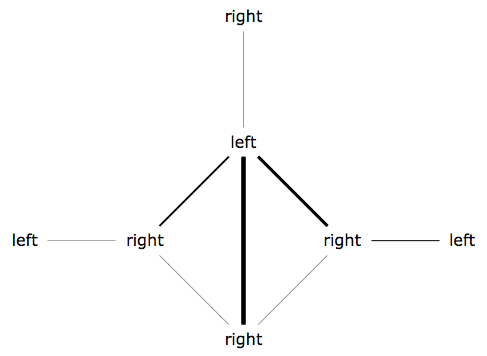
\includegraphics[width=8cm, height=6cm]{taking-sides-graph.png}\\
  \caption{Grafo extraído de \cite{malouf-taking_sides}. Os vértices são usuários e as arestas, citações entre eles. Arestas mais escuras indicam frequência de citação mais alta.}
  \label{fig:malouf}
\end{figure}


Padrões de citação entre documentos também foram investigados em \cite{efron}. Neste artigo, os experimentos envolvem dois \emph{datasets}: o primeiro é composto de artigos políticos Estadunidenses de Direita ou Esquerda, coletados em \emph{sites} e \emph{blogs} políticos - explicitamente partidários ou não -; o segundo é composto de textos retirados de \emph{sites} de artistas musicais, divididos entre as categorias Alternativo e Popular. As taxas de acerto relatadas para as aplicações de Naïve Bayes nestes corpora foram, respectivamente, 64.71\%e 50.1\%. Um SVM padrão foi aplicado apenas ao primeiro \emph{dataset}, pois não havia recursos computacionais suficientes para a aplicação no segundo. A taxa de acerto verificada foi significativamente melhor: 72.96\%. A fim de melhorar as taxas de acerto na classificação dos documentos, \cite{efron} estima a perspectiva de cada um deles avaliando a probabilidade de que eles sejam co-citados com documentos referência de cada perspectiva. Para o primeiro corpus, a metodologia relatada é a seguinte:

\begin{enumerate}
  \item Duas listas de URLs são criadas: uma contendo \emph{sites} referência de Esquerda; outra, de Direita;
  \item para cada documento \emph{d\_i}, computa-se sua probabilidade de ser co-citado com alguma URL da lista de Direita e, em seguida, com alguma da lista de Esquerda;
  \item se a razão entre estas probabilidades for maior que 1, o documento é classificado como de Direita; caso seja menor que 1, como de Esquerda.

\end{enumerate}

As probabilidades foram computadas com o auxílio do buscador Altavista, que fornecia o número de documentos indexados que citavam, simultaneamente, \emph{d\_i} e alguma das URLs das listas de referência. Esta metodologia, aplicada ao primeiro \emph{dataset}, resultou em uma taxa de acerto de 94.1\%. No segundo \emph{dataset}, o procedimento foi análogo: as listas de URLs foram divididas entre Alternativo e Popular. A taxa de acerto máxima obtida foi de 88.84\%.

Todos os artigos que propuseram metodologias para melhorar a classificação em corpora com vocabulário muito uniforme consideraram algum esquema de citação. Se o corpus for composto de documentos pouco citados na Web, o esquema de \cite{efron} pode não trazer nenhuma melhoria significativa ao problema. Se os autores dos documentos não mencionarem significativamente um ao outro, como aconteceu nos debates estudados por \cite{aaai-politics} e \cite{malouf-taking_sides}, a metodologia explorada por estes trabalhos também não pode ser empregada. Essa área de pesquisa, portanto, ainda tem alguns problemas em aberto - e, considerando que estes três artigos foram escritos há mais de quatro anos, ela não parece atrair muita atenção. A justificativa para isso, provavelmente, tem a ver com o fato de que uniformidade no vocabulário não é um problema tão comum em Mineração de Perspectiva. No \textbf{capítulo X}, técnicas envolvendo comparação entre documentos, que podem trazer benefícios à classificação de \emph{datasets} difíceis, como aqueles em que o vocabulário é mais uniforme, serão discutidas.

\section{Conclusão}

Este capítulo apresentou a ideia de que pessoas costumam utilizar palavras específicas para defender perspectivas diferentes. O uso de classificadores baseados na presença ou frequência das palavras, portanto, costuma ser indicado para a identificação dessas perspectivas. Entretanto, em alguns casos, essa ideia não se confirma: as perspectivas defendidas se apóiam mais nas construções do discurso do que no uso de palavras específicas. Naturalmente, as taxas de acerto desses classificadores, nestes casos, são menores do que o desejado. Experimentos com o modelo de tópicos L-LDA foram conduzidos, conduzindo à visualização parcial de como palavras, em dois \emph{datasets} diferentes, se relacionam com diferentes perspectivas. No primeiro \emph{dataset}, as palavras listadas para cada perspectiva se relacionam, semanticamente, melhor com a perspectiva em si do que no segundo \emph{dataset}. Neste último, palavras genéricas, como artigos e conjunções, se associam muito fortemente a todas as perspectivas, colaborando para uma uniformização do vocabulário. Isto explica, ainda que não seja trivial avaliar o quanto, as taxas de acerto mais altas obtidas com um Naïve Bayes no primeiro \emph{dataset}.

Por fim, este capítulo também revisa artigos que discutem a questão do vocabulário do corpus. Estes artigos propõem metodologias para melhorar a classificação em \emph{datasets} cujo vocabulário é considerado muito uniforme. Pouca pesquisa tem sido feita nesta direção - provavelmente porque o problema é pouco comum.
 
%o primeiro \emph{dataset}, os artigos estão escritos sob uma das seguintes perspectivas: pró-Palestina ou pró-Israel. Por conta disso, o tópico \emph{pal} foi atribuído a todos os documentos pró-Palestina e o tópico \emph{isr}, a todos os pró-Israel. Estes tópicos facilitam a visualização das palavras mais fortemente associadas a cada uma das duas perspectivas, de acordo com o vocabulário empregado nos artigos. Um terceiro tópico, \emph{gen}, foi atribuído a todos os documentos, a fim de capturar as palavras que co-ocorrem neles independentemente de suas perspectivas. Após a execução do modelo, as 100 palavras mais fortemente associadas a cada um dos 3 tópicos foram coletadas. 35\% das associadas a \emph{isr} não estão presentes no conjunto recolhido para \emph{gen}. Para \emph{pal}, essa percentagem cai para 29\%. Por fim, 32\% das palavras mais fortemente associadas a \emph{isr} não fazem parte das 100 palavras mais fortemente associadas a \emph{pal} e vice-versa. Essas percentagens indicam que os autores dos documentos pró-Israel utilizam um vocabulário ligeiramente mais específico, na defesa de seus pontos de vista, do que os autores pró-Palestina. É importante ressaltar que nenhuma palavra foi filtrada na análise - ou seja, termos muito frequentes como \emph{the}, \emph{of} e \emph{and}, comumente extraídos dos \emph{datasets} antes da etapa de classificação, estavam presentes nos documentos processados pelo L-LDA.    

%Palavras associadas a \emph{isr} que não foram associadas a \emph{gen}
%['arafat', 'be', 'some', 'roadmap', 'us', 'yet', 'out', 'sharon', 'ariel', 'support', 'three', 'bush', 'palestine', 'new', 'terrorism', 'leader', 'then', 'jewish', 'after', 'arab', 'leadership', 'plan', 'president', 'than', 'bank', 'prime', 'regarding', 'like', 'could', 'violence', 'against', 'while', 'time', 'american', 'first']

%Palavras associadas a \emph{pal} que não foram associadas a \emph{gen}
%['then', 'some', 'authority', 'against', 'occupied', 'negotiations', 'occupation', 'sharon', 'united', 'end', 'way', 'palestine', 'international', 'be', 'after', 'plan', 'president', 'law', 'those', 'prime', 'land', 'i', 'violence', 'us', 'q', 'while', 'time', 'situation', 'first']

%Palavras associadas a \emph{pal} que não foram associadas a \emph{isr}
%['because', 'people', 'authority', 'states', 'right', 'occupied', 'any', 'negotiations', 'occupation', 'what', 'united', 'end', 'also', 'been', 'their', 'other', 'way', 'international', 'law', 'do', 'which', 'government', 'very', 'they', 'now', 'those', 'about', 'land', 'these', 'q', 'i', 'situation']

%Palavras associadas a \emph{isr} que não foram associadas a \emph{pal}
%['arafat', 'into', 'settlements', 'years', 'yet', 'out', 'even', 'would', 'ariel', 'west', 'support', 'three', 'bush', 'gaza', 'new', 'terrorism', 'leader', 'we', 'jewish', 'arab', 'most', 'leadership', 'minister', 'roadmap', 'than', 'bank', 'both', 'regarding', 'like', 'could', 'war', 'american']
%\textbf{As palavras estão ordenadas de acordo com a força da associação com cada um dos tópicos}


%\textbf{Lista de palavras e desempenho. Imagens e tabelas.}

%Dado que em boa parte dos artigos estudados neste projeto, como \cite{lin-et-al2006} e \cite{klebanov}, atinge-se taxas de acerto superiores a 80\% com classificadores baseados em frequência de palavras, conclui-se que a mineração de perspectivas em discussões, artigos opinativos e debates requer metodologias diferentes, a depender de como as palavras foram escolhidas pelos autores dos documentos. %Nos debates estudados por \cite{hirst-et-al}, expressões de ataque e defesa são mais frequentes do que \emph{stigma words} e, como o método empregado no artigo foi um SVM treinado com frequências de palavras, observou-se que a classificação obtida para os lados do debate não refletia as perspectivas \emph{liberal} ou \emph{conservadora} - mas sim os lados \emph{oposição} (expressões de ataque) e \emph{situação} (expressões de defesa). 
%Estes estudos indicam a possibilidade de que, em debates e discussões nos quais há uma homogeneização do vocabulário empregado - o que pode acontecer quando todos os lados utilizam, em proporções similares, tanto expressões de ataque quanto de defesa -, classificadores baseados exclusivamente nas palavras utilizadas e/ou em suas frequências apresentarão má performance.

%A avaliação do desempenho desses classificadores\footnote{\textbf{SVMs e Naive Bayes padrão; LSPM}} nos \emph{datasets} estudados revela que artigos opinativos e notícias consolidaram perspectivas, através da escolha do vocabulário utilizado, melhor do que debates. Apesar disso, uma generalização neste sentido, restringindo o uso desses classificadores a artigos e notícias, não é recomendada por falta de indicativos linguísticos que comprovem essa tendência. Uma estratégia que pode ajudar na escolha ou descarte de um classificador desse tipo é uma análise das palavras que estão contidas nos documentos.

%\textbf{mostrar as percentagens prum dataset onde a linguagem eh mais uniforme. discutir.} 
%Explicar q isso nunca foi feito e q pessoas q ncontraram merda com essa feature fizeram outras coisas. descrever essas coisas.

%Estas hipóteses ilustram  
%Como indica \cite{}: 

%\textbf{MODO RASCUNHO AINDA}

%Explicar que uma diferença fundamental notada entre os datasets observados diz respeito à formalidade da linguagem empregada nos documentos. Enquanto alguns datasets utilizam documentos provenientes de meios onde a norma culta da linguagem impera, e uma revisão ortográfica é utilizada, outros são carregados de gírias, expressões e abreviações típicas da linguagem da Internet e contêm, eventualmente, grafias erradas para uma mesma palavra. <Dar exemplos textuais. Mostrar uma tabelinha, algo assim, indicando o volume de datasets com linguagem informal nos documentos estudados.> 

%A linguagem informal pode criar alguns desafios para a Mineração de Perspectiva [FECHAR O PROBLEMA EM: IDENTIFICAÇÃO DA PERSPECTIVA PRESENTE EM UM DOCUMENTO], especificamente no que diz respeito ao pré-processamento dos documentos e à escolha do método empregado. No pré-processamento, como indicado em (aaai-politics.pdf e 10.1.1.138.7160.pdf), a correção gramatical das palavras é bastante indicada. Com uma única versão de grafia para cada palavra (a correta), diminui-se a quantidade de ruído que grafias erradas podem causar na classificação.

%Uma característica dos datasets que deveria ser considerada sempre antes de se escolher o método utilizado - mas não é prática entre as pessoas que estudam perspective mining - é a frequência das palavras nos documentos do dataset. Se o léxico empregado pelos autores dos textos muda sensivelmente a depender de sua ideologia/perspectiva defendida/ponto de vista, é possível resolver o problema utilizando classificadores que usam essa frequencia como feature. GASTE TEMPO DANDO ALGUNS EXEMPLOS.  Em datasets informais, entretanto, como aponta Efron, a linguagem empregada por todos os lados da discussão pode ser basicamente a mesma: termos com forte carga de polaridade e gírias/jargões comuns na discussão [EXEMPLO]. Neste caso, é preciso utilizar métodos que utilizem mecanismos mais rebuscados do que a simples frequência/presença das palavras no texto. Alguns autores utilizam métodos mais gramaticais para lidar com datasets informais, como é o caso de , BLE e BLI. Os 2 primeiros criam o conceito de Opinion Frame (DEFINIR O CONCEITO). No primeiro caso, a ideia é associar corretamente opiniões a alvos, e associar alvos iguais utilizando técnicas de co-referência. Segundo Wiebe et al. (pegar a citação corretamente), ter as targets associadas, com as opiniões próximas, é uma boa forma de entender o overall de opiniões de um documento. A estratégia é uma alternativa possível para documentos em que as perspectivas estão muito associadas à linguagem opinativa, e onde essa linguagem é comum para todos os lados. Infelizmente, os resultados alcançados indicam que a tarefa não é trivial: blablablablababla (resolver coreferencia pra linkar targets não é tão simples assim => e dê exemplo). 

%uma diferença fundamental notada entre os \emph{datasets} observados diz respeito à formalidade da linguagem empregada nos documentos. Enquanto alguns datasets utilizam documentos provenientes de meios onde a norma culta da linguagem impera, e uma revisão ortográfica é utilizada, outros são carregados de gírias, expressões e abreviações típicas da linguagem da Internet e contêm, eventualmente, grafias erradas para uma mesma palavra. <Dar exemplos textuais. Mostrar uma tabelinha, algo assim, indicando o volume de datasets com linguagem informal nos documentos estudados.> 

